\documentclass[11pt]{beamer}
\usepackage[utf8]{inputenc}
\usepackage[T1]{fontenc}


\usepackage[backend=bibtex,style=authoryear]{biblatex}
\addbibresource{EDA.bib}

%% End of citations additions

%\usetheme{AnnArbor}
%\usetheme{Antibes}
%\usetheme{Berkeley}
%\usetheme{Berlin}
%\usetheme{boxes}
%\usetheme{Darmstadt}
%\usetheme{default}
%\usetheme{Frankfurt}
%\usetheme{Ilmenau}
%\usetheme{JuanLesPins}
\usetheme{Luebeck}
%\usetheme{Malmoe}
%\usetheme{Montpellier}
%\usetheme{PaloAlto}
%\usetheme{Rochester}
%\usetheme{Singapore}
%\usetheme{Szeged}

\setbeamertemplate{footline}
{%
	\leavevmode%
	\hbox{\begin{beamercolorbox}[wd=.2\paperwidth,ht=2.5ex,dp=1.125ex,leftskip=.3cm,rightskip=.3cm plus1fill]{author in head/foot}%
			\usebeamerfont{author in head/foot} \insertframenumber{} / \inserttotalframenumber
		\end{beamercolorbox}%
		\begin{beamercolorbox}[wd=.3\paperwidth,ht=2.5ex,dp=1.125ex,leftskip=.3cm plus1fill,rightskip=.3cm]{author in head/foot}%
			\usebeamerfont{author in head/foot}\insertshortauthor
		\end{beamercolorbox}%
		\begin{beamercolorbox}[wd=.5\paperwidth,ht=2.5ex,dp=1.125ex,leftskip=.3cm,rightskip=.3cm plus1fil]{title in head/foot}%
			\usebeamerfont{title in head/foot}\insertshorttitle
	\end{beamercolorbox}}%
	\vskip0pt%
}
\setbeamertemplate{headline}{}

\begin{document}
	\author{Gary R Seamans}
	\title{R Exploratory Data Analysis}
	\subtitle{R Brown Bag Series \#3}
	%\logo{\scalebox{0.035}{
\includegraphics{R_logo.png}}}
	\institute{The MITRE Corporation}
	%\date{}
	%\subject{}
	%\setbeamercovered{transparent}
	%\setbeamertemplate{navigation symbols}{}
	\begin{frame}[plain]
		\maketitle
    \end{frame}

\begin{frame}{
	\begin{minipage}[t]{0.55\textwidth}
		Agenda
	\end{minipage}
	\hfill
	\begin{minipage}[t]{0.35\textwidth}
		\flushright
		\scalebox{0.035}{
\includegraphics{R_logo.png}}
	\end{minipage}
}{}
%% ==================== Content ===========================%%
\begin{center}
	\begin{itemize}
		\item What is EDA?
		\item Demonstrations
		\item Questions
	\end{itemize}
\end{center}
\end{frame}

%% Overview ===================
\begin{frame}{
	\begin{minipage}[t]{0.55\textwidth}
		Overview -What is EDA?
	\end{minipage}
	\hfill
	\begin{minipage}[t]{0.35\textwidth}
		\flushright
		\scalebox{0.035}{
\includegraphics{R_logo.png}}
	\end{minipage}
}{}
%% ==================== Content ===========================%%

	Exploratory Data Analysis (EDA) is an approach/philosophy for data analysis that employs a variety of techniques (mostly graphical) to:
	
	\begin{itemize}
		\item maximize insight into a data set
		\item uncover underlying structure
		\item extract important variables
		\item detect outliers and anomalies
		\item test underlying assumptions
		\item develop parsimonious models
		\item determine optimal factor settings
	\end{itemize}
\colorbox{yellow}{\parencite{whatiseda}}
\end{frame}

%% Overview What is EDA Seminal work ===================
\begin{frame}{
	\begin{minipage}[t]{0.55\textwidth}
		What is EDA contd.
	\end{minipage}
	\hfill
	\begin{minipage}[t]{0.35\textwidth}
		\flushright
		\scalebox{0.035}{
\includegraphics{R_logo.png}}
	\end{minipage}
}{}
%% ==================== Content ===========================%%

	The seminal work on EDA is by John Tukey \parencite{tukey1977}. It is very readable and still relevant. Another excellent book is Understanding Robust and Exploratory Data Analysis \parencite{HoaglinUnderstandingrobustexploratory1983}  
	\vspace{0.5cm}
	
	 \href{http://www.itl.nist.gov/div898/handbook/eda/section1/eda11.htm}{\textcolor{blue}{\underline{Engineering Statistics Handbook (NIST)}}} is another good reference.

\end{frame}

%% Overview  Tidy Data ===================
\begin{frame}{
	\begin{minipage}[t]{0.55\textwidth}
		EDA Examples
	\end{minipage}
	\hfill
	\begin{minipage}[t]{0.35\textwidth}
		\flushright
		\scalebox{0.035}{
\includegraphics{R_logo.png}}
	\end{minipage}
}{}
%% ==================== Content ===========================%%
All of the examples demonstrate data loading, cleaning, exploratory data analysis, and a final analysis.
\begin{itemize}
	\item Old Faithful
	\item Music
	\item On-time Arrivals
	\item Credit Card Default
\end{itemize}

\end{frame}



%% Old Faithful  ===================
\begin{frame}{
	\begin{minipage}[t]{0.55\textwidth}
		Old Faithful
	\end{minipage}
	\hfill
	\begin{minipage}[t]{0.35\textwidth}
		\flushright
		\scalebox{0.035}{
\includegraphics{R_logo.png}}
	\end{minipage}
}{}
%% ==================== Content ===========================%%
In this example we'll look at the eruptions of Old Faithful and see if there is a correlation between
the length of the eruption and the time until the next eruption.
\begin{center}
	\scalebox{0.5}{\includegraphics{Oldfaithful.jpeg}}
\end{center}
\end{frame}


%% Music ===================
\begin{frame}{
	\begin{minipage}[t]{0.55\textwidth}
		Music
	\end{minipage}
	\hfill
	\begin{minipage}[t]{0.35\textwidth}
		\flushright
		\scalebox{0.035}{
\includegraphics{R_logo.png}}
	\end{minipage}
}{}
%% ==================== Content ===========================%%
This example takes music listeners preferences and does market basket analysis using association mining rules.
\begin{center}
	\scalebox{0.5}{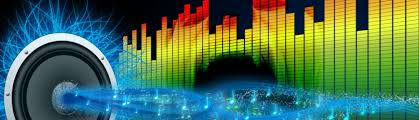
\includegraphics{music.jpeg}}
\end{center}
\end{frame}

%% On-time Arrivals ===================
\begin{frame}{
	\begin{minipage}[t]{0.55\textwidth}
		On-time arrivals
	\end{minipage}
	\hfill
	\begin{minipage}[t]{0.35\textwidth}
		\flushright
		\scalebox{0.035}{
\includegraphics{R_logo.png}}
	\end{minipage}
}{}
%% ==================== Content ===========================%%
An example of analyzing on-time arrivals for a small number of airports.

\begin{center}
	\scalebox{0.5}{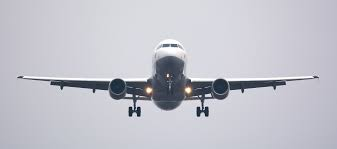
\includegraphics{airplane.jpeg}}
\end{center}
\end{frame}

%% Credit Card Default ===================
\begin{frame}{
	\begin{minipage}[t]{0.55\textwidth}
		Credit Card Default
	\end{minipage}
	\hfill
	\begin{minipage}[t]{0.35\textwidth}
		\flushright
		\scalebox{0.035}{
\includegraphics{R_logo.png}}
	\end{minipage}
}{}
%% ==================== Content ===========================%%
Credit card default is a big problem for banks. This example shows how you might go about
predicting who will default.
\begin{center}
	\scalebox{0.5}{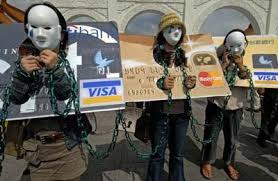
\includegraphics{default.jpeg}}
\end{center}
\end{frame}

%% Questions ===================
\begin{frame}{
	\begin{minipage}[t]{0.55\textwidth}
		Questions
	\end{minipage}
	\hfill
	\begin{minipage}[t]{0.35\textwidth}
		\flushright
		\scalebox{0.035}{
\includegraphics{R_logo.png}}
	\end{minipage}
}{}
%% ==================== Content ===========================%%
\begin{center}
	
\end{center}
\end{frame}



%%===================== Citations =================================%%
\appendix
\begin{frame}[allowframebreaks]{References}{}
\footnotesize
\printbibliography

\end{frame}
\end{document}